\chapter{Results}
\label{chap:results}
\section{Decision trees}
From the implementation of a decision tree, we get the following segments and the respective warning signs for each segment.
\begin{itemize}
\item[*] \textbf{Segment 1:}
Income lower or equal than 5.000.000 and assets, lower or equal than 50.000.000.

\begin{figure}[htbp]
  \centering
  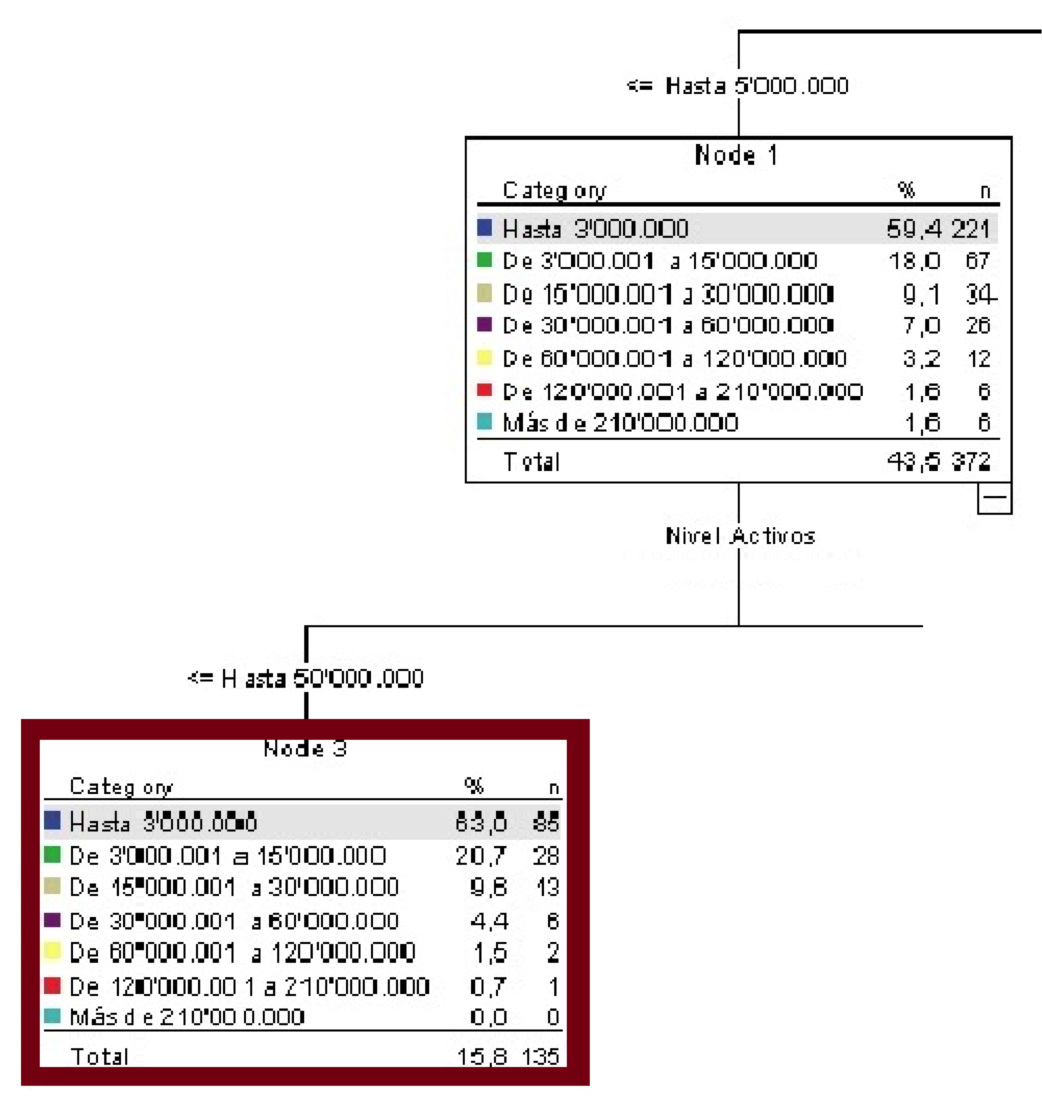
\includegraphics[width=0.95\textwidth]{Segmento1}
  \caption{caption}
  \label{fig:label}
\end{figure}

The warning sign for this segment is the transactions made by the costumers above 2.500.000 per month.  16.2\% of the customers in the segment 1, made transactions over 2.500.000.
\item[*] \textbf{Segment 2:}
Income lower or equal than 5.000.000 and assets between 50.000.000 and 300.000.000.

\begin{figure}[htbp]
  \centering
  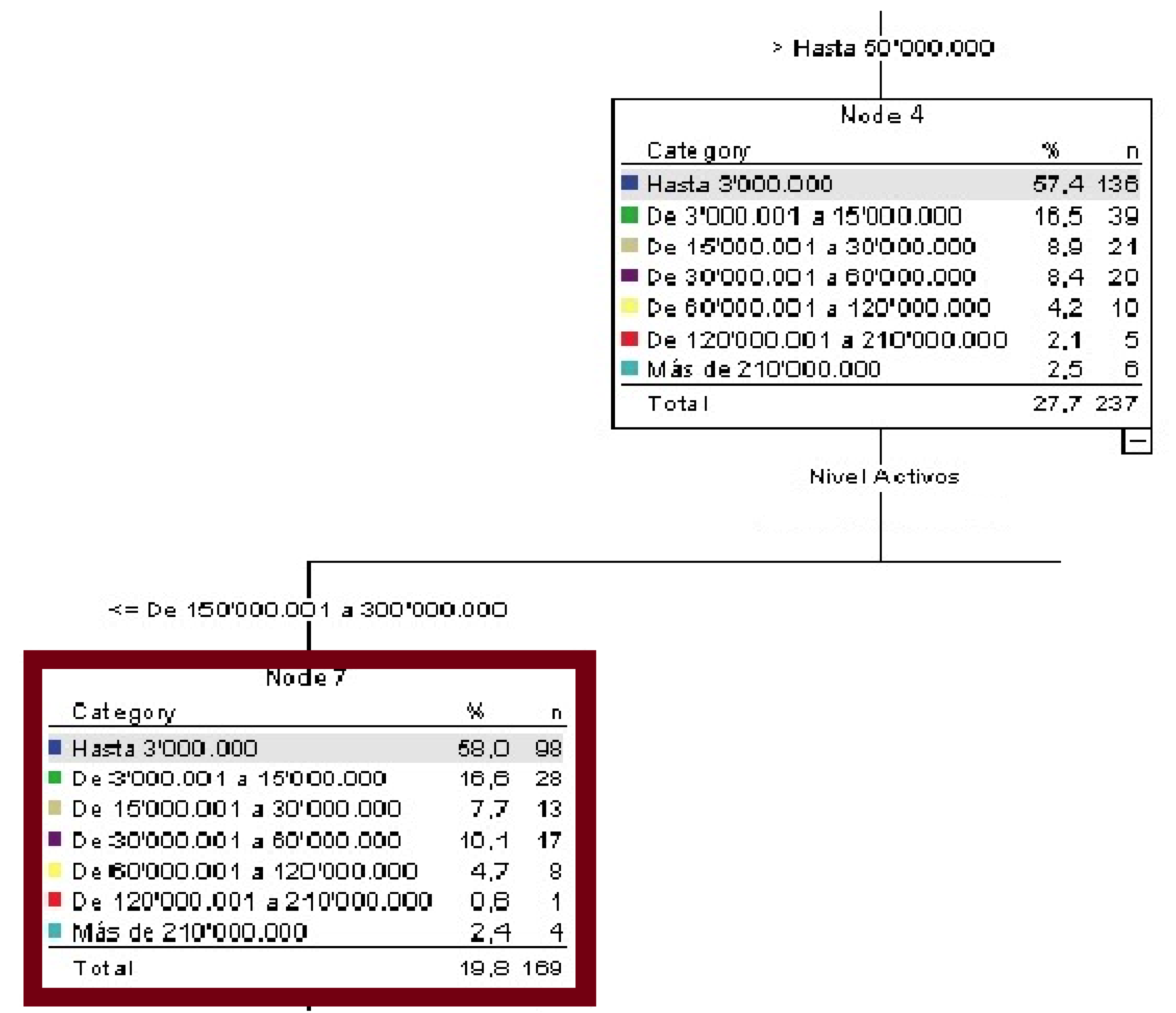
\includegraphics[width=0.95\textwidth]{Segmento2}
  \caption{caption}
  \label{fig:label}
\end{figure}

The warning sign for this segment is the transactions made by the customers above 5.000.000 per month.  17.8\% of the customers in the segment two, made transactions over 5.000.000.
\item[*] \textbf{Segment 3:}
Income lower or equal than 5.000.000 and assets more than 300.000.000.

\begin{figure}[htbp]
  \centering
  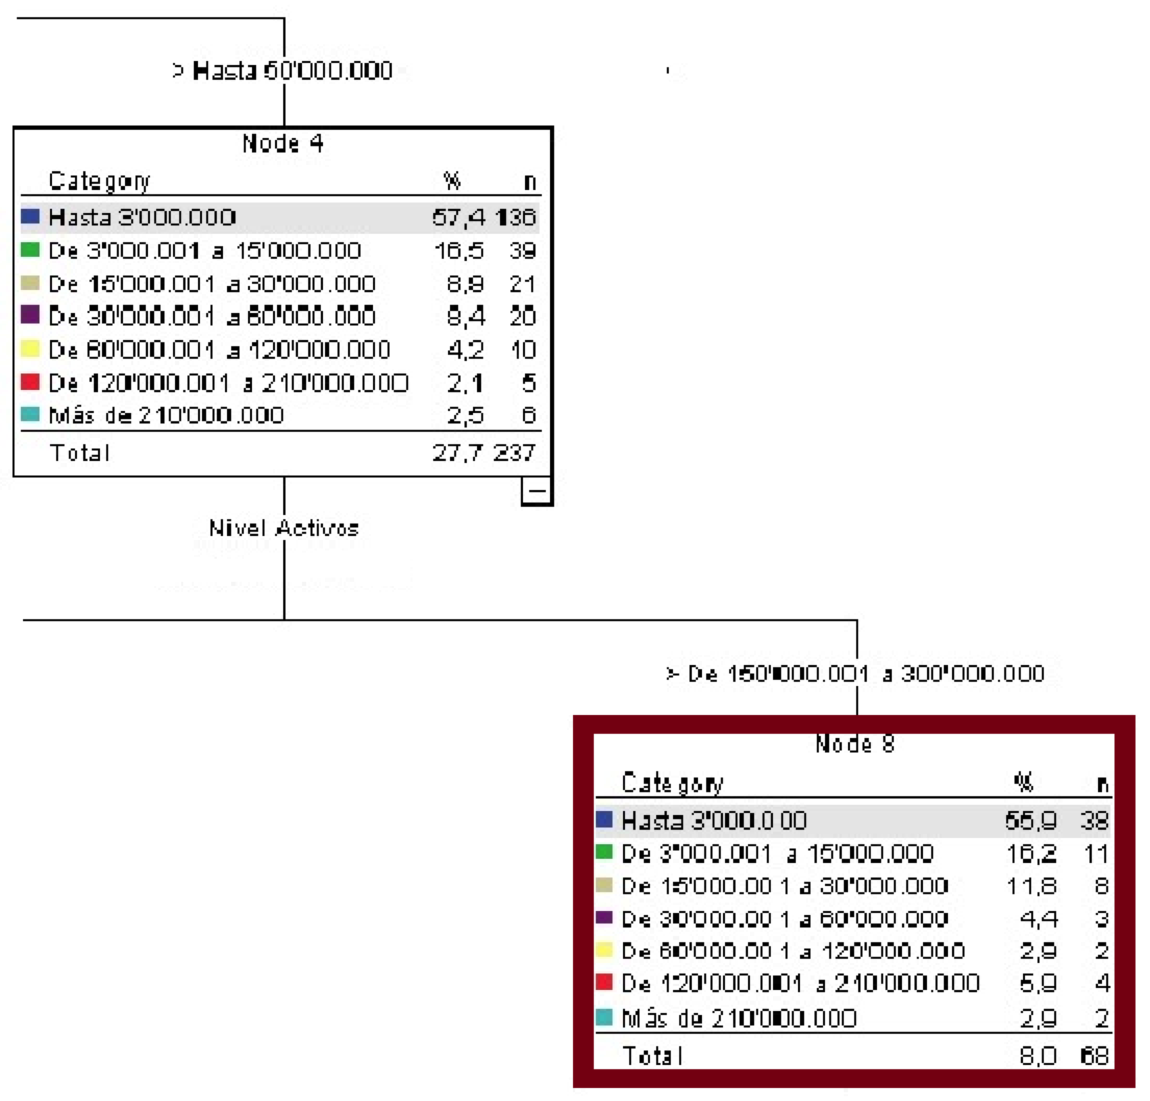
\includegraphics[width=0.95\textwidth]{Segmento3}
  \caption{caption}
  \label{fig:label}
\end{figure}

The warning signs for this segment are: \begin{itemize}
\item[*] Transactions made by the customers above 10.000.000 per month, or
\item[*] customers that they have assets more than 1.000.000.000.
\end{itemize}
11.7\% of the customers in the segment 3, made transactions over 10.000.000 and 14.7\% of the customers in segment 3, have assets more than 1.000.000.000.
\item[*] \textbf{Segment 4:}
Income more than 5.000.000 and assets, lower or equal than 150.000.000.
\begin{figure}[htbp]
  \centering
  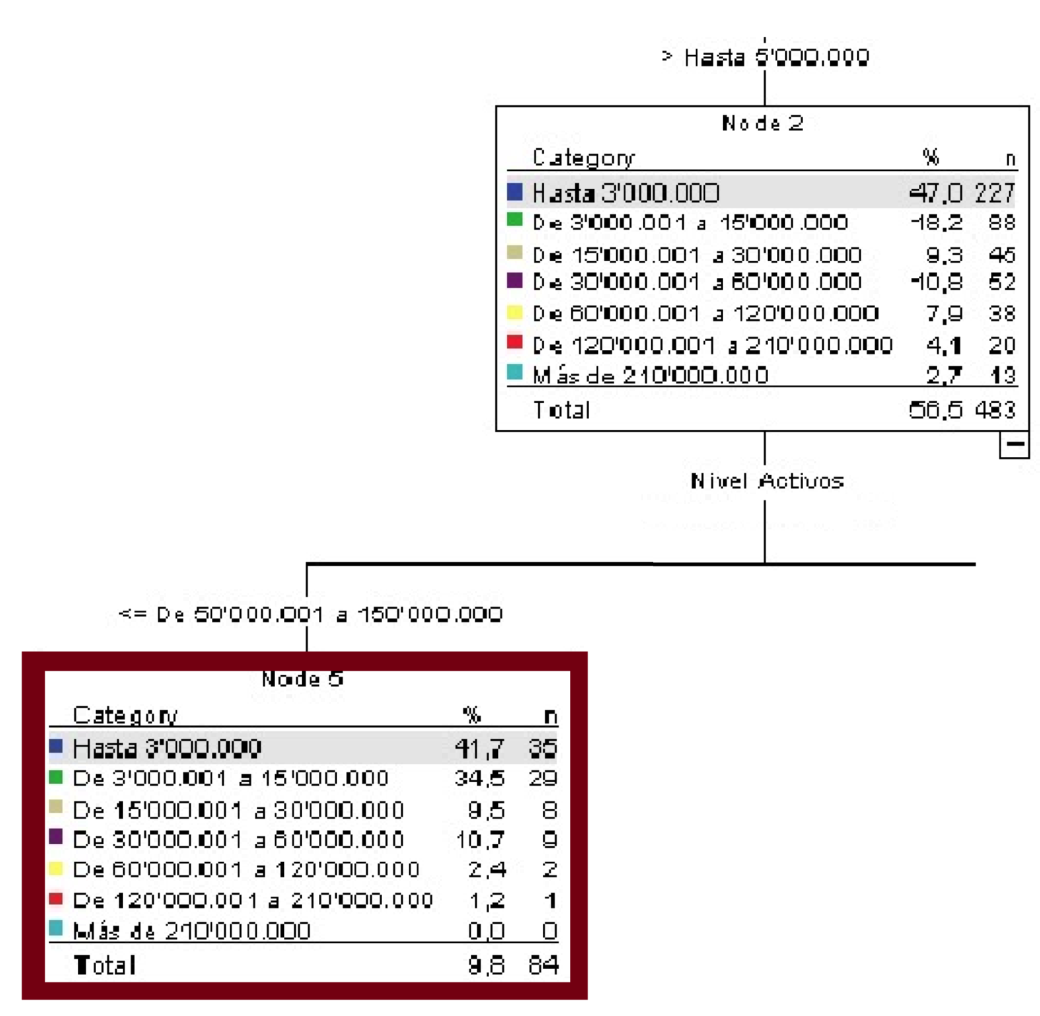
\includegraphics[width=0.95\textwidth]{Segmento4}
  \caption{caption}
  \label{fig:label}
\end{figure}
The warning sign for this segment is the transactions made by the customers above 10.000.000.  3.6\% of the customers in segment 4, made transactions over 10.000.000 per month.
\item[*] \textbf{Segment 5:}
Income more than 5.000.000 and assets between 150.000.000 and 300.000.000.
\begin{figure}[htbp]
  \centering
  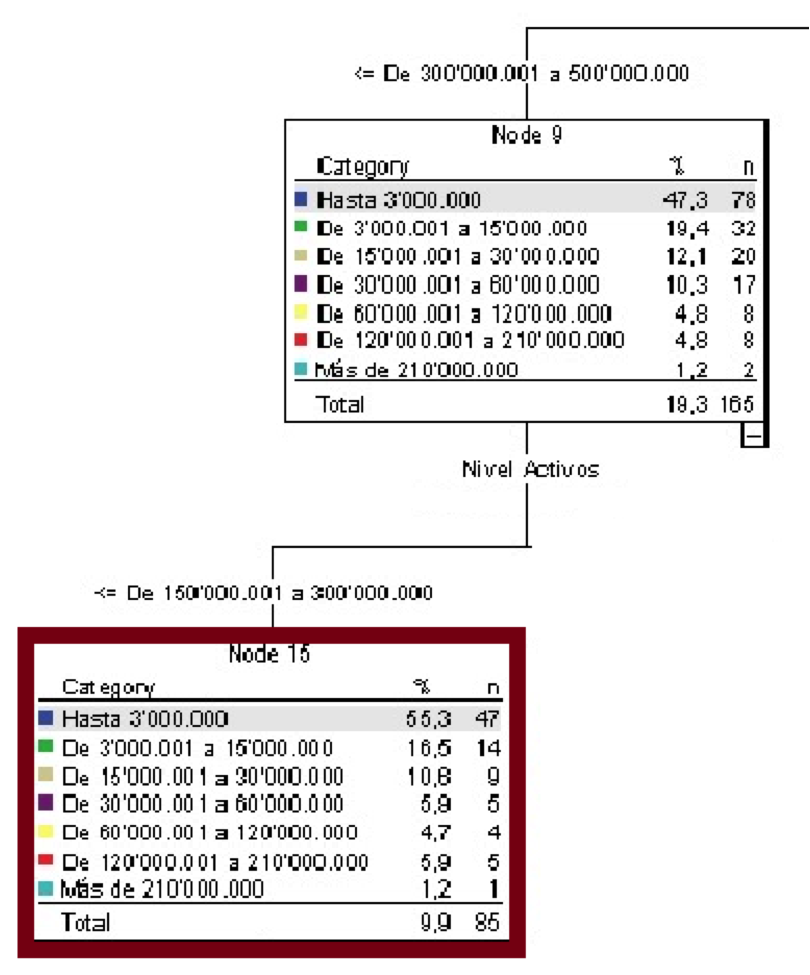
\includegraphics[width=0.95\textwidth]{Segmento5}
  \caption{caption}
  \label{fig:label}
\end{figure}
The warning sign for this segment is the transactions made by the customers above 20.000.000 per month.  7.1\% of the customers in the segment 5, made transactions over 20.000.000.
\item[*] \textbf{Segment 6:}
Income more than 5.000.000 and assets between 300.000.000 and 500.000.000.
\begin{figure}[htbp]
  \centering
  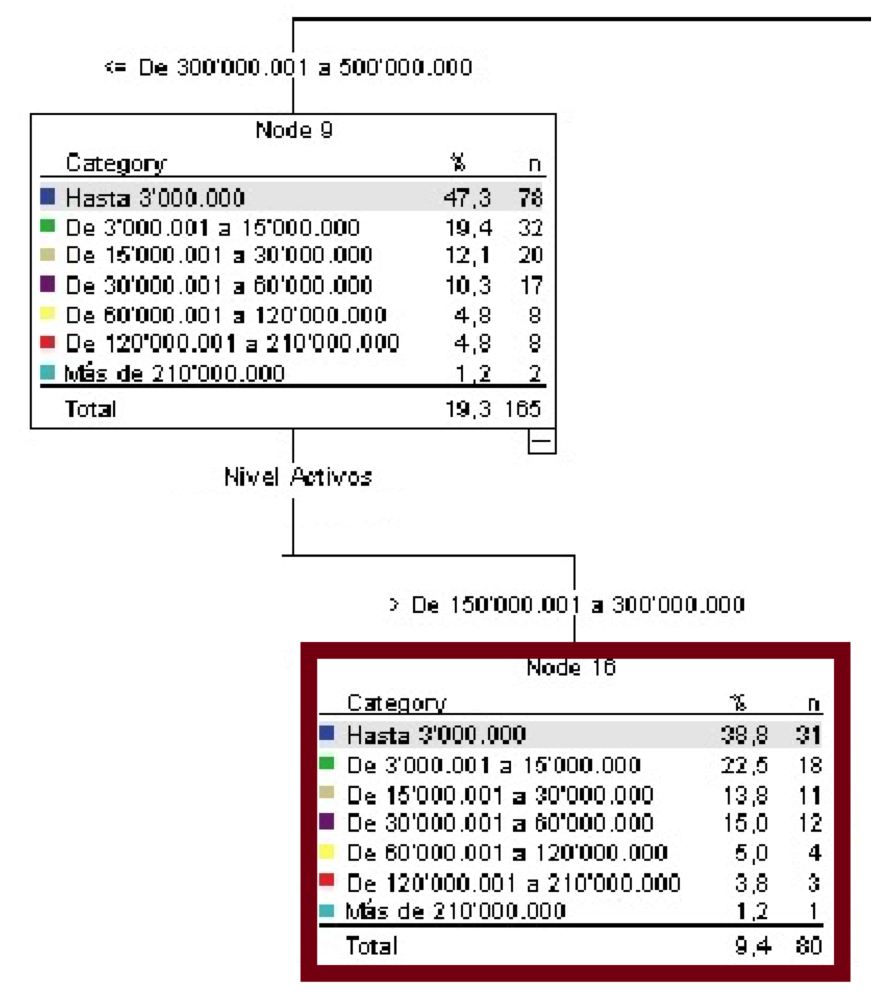
\includegraphics[width=0.95\textwidth]{Segmento6}
  \caption{caption}
  \label{fig:label}
\end{figure}
The warning sign for this segment is the transactions made by the customers above 20.000.000 per month.  4.8\% of the customers in the segment 6, made transactions over 20.000.000.
Another warning sign for this segment is the customers, which economic activity is housewives, 2,5\% of the segment 6, and business associate, 1,2\% of the segment 6.
\item[*] \textbf{Segment 7:}
Income between 5.000.000 and 10.000.000 and assets more than 500.000.000
\begin{figure}[htbp]
  \centering
  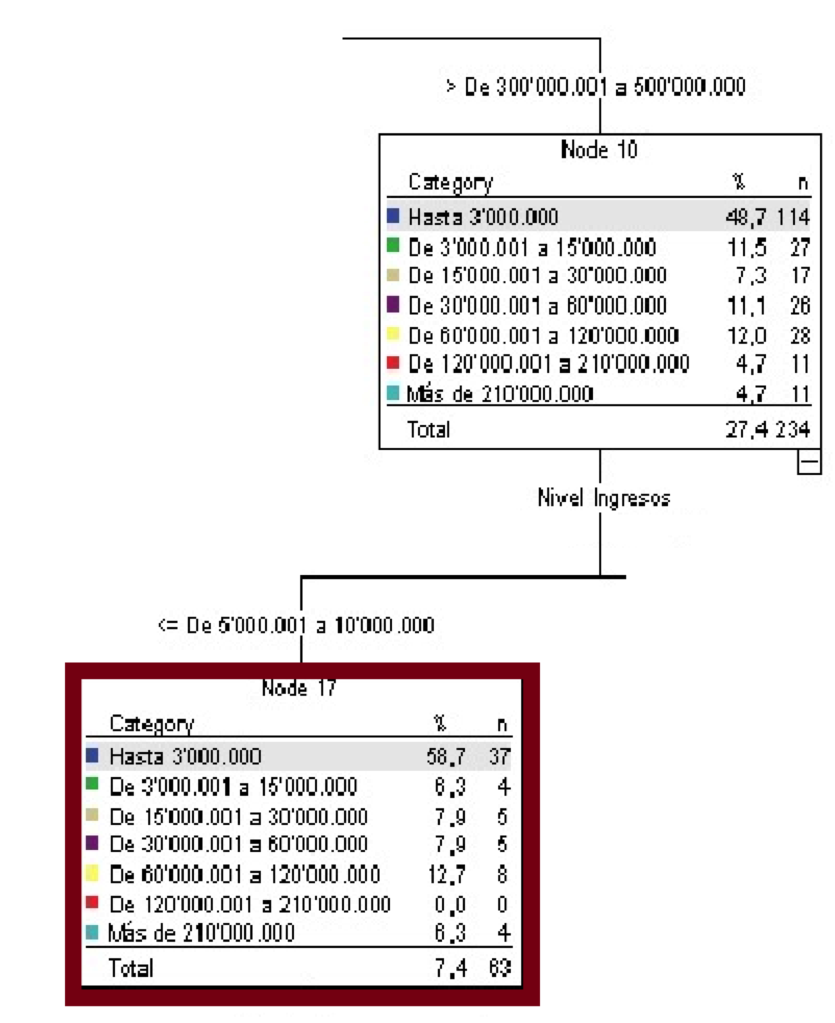
\includegraphics[width=0.95\textwidth]{Segmento7}
  \caption{caption}
  \label{fig:label}
\end{figure}
The warning sign for this segment is the transactions made by the customers above 35.000.000 per month.  6.35\% of the customers in the segment 7, made transactions over 35.000.000.
Another warning sign for this segment is the customers, which economic activity is a business associate, 4.76\% of the segment 7.
\item[*] \textbf{Segmento 8:}
Income more than 10.000.000 and assets more than 500.000.000.
\begin{figure}[htbp]
  \centering
  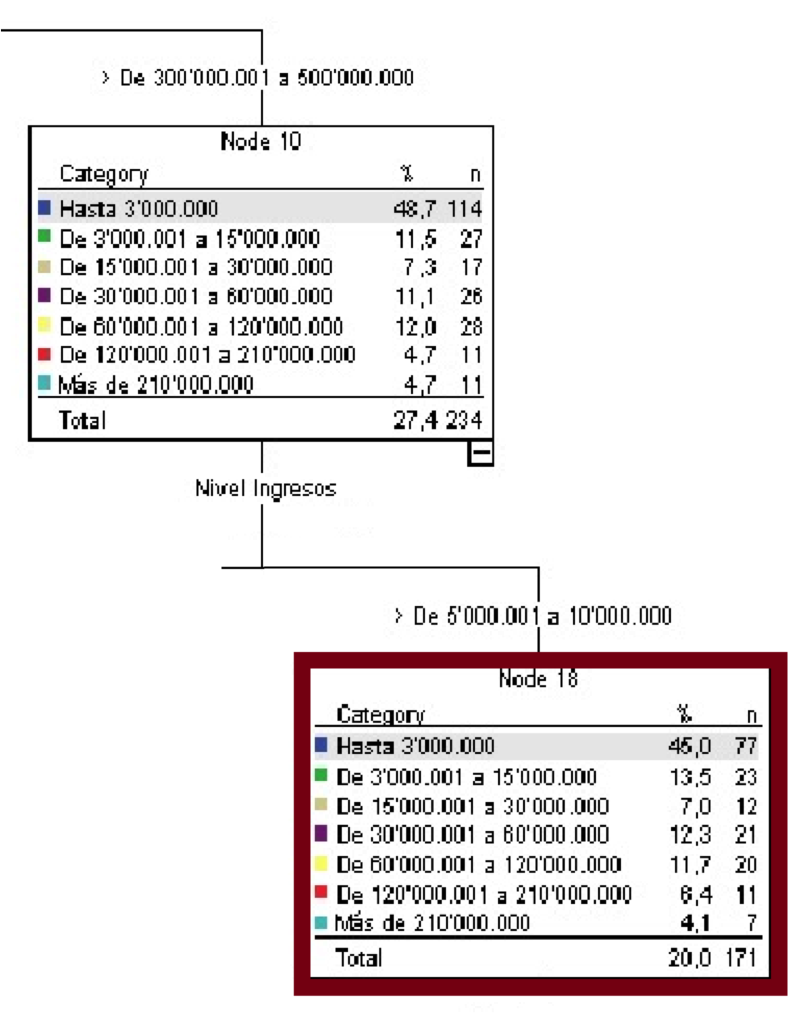
\includegraphics[width=0.95\textwidth]{Segmento8}
  \caption{caption}
  \label{fig:label}
\end{figure}
The warning sign for this segment is the transactions made by the customers above 35.000.000 per month.  4.1\% of the	 customers in the segment 8, made transactions over 35.000.000.
Another warning sign for this segment is the customers, which economic activity is a housewife, 6.43\% of the segment 8.
\end{itemize}
\section{K-Means Algorithm}
Since the implementation of a K-means, we get the following segments and the respective warning signs for each segment.
\begin{itemize}
\item[*] \textbf{Segment 1:}
Assets more than 300.000.000 and income more than 20.000.000.
The warning sign for this segment is the transactions made by the customers above 34.000.000 per month. 5.12\% of the customers in this segment made transactions over 34.000.000.
\item[*] \textbf{Segment 2:}
Assets between 150.000.000 and 500.000.000, and income between 10.000.000 and 50.000.000.
The warning sign for this segment is the transactions made by the customers above 10.000.000 per month. 11.62\% of the customers in this segment made transactions over 10.000.000.
\item[*] \textbf{Segment 3:}
Assets lower or equal than 150.000.000 and income lower or equal than 10.000.000.
The warning sign for this segment is the transactions made by the customers above 18.000.000 per month. 1.31\% of the customers in this segment, made transactions over 18.000.000.
\end{itemize}
\clearemptydoublepage
